\section{Multiple Layers}
\label{Sec: Multiple Layers}

In \cite{Nicholls16b}, the author discusses how to apply our HOPS methodology in multilayered configurations. He considers a multilayered material with $M$ (finite) interfaces at 
$$z=a^{(m)}+g^{(m)}(x,y),\quad 1\leq m \leq M,$$
which are $d_x \times d_y$ periodic
$$g^{(m)}(x+d_x,y+d_y)=g^{(m)}(x,y),\quad 1\leq m \leq M,$$
separating $(M+1)$--many layers.
%\vspace{-12mm}
\begin{figure}[H]
    \centering
    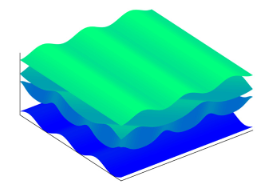
\includegraphics[width=7.6cm]{sections/7_conclusions_and_future_directions/multilayered.png}%
    \vspace{3mm}
    \caption{A five--layer problem configuration with layer interfaces $z = a^{(m)}+g^{(m)}(x).$}%
    \label{fig:example}%
\end{figure}
\vspace{-15mm}
%\begin{flushleft}
A generalization of our analyticity theorems (cf. $\S 4.5$) up to $M$ parameters is included as Theorem~$3.2$ in \cite{Nicholls16b}. For this, we consider quite general systems of linear equations of the form
%\end{flushleft}
\be
\bA(\tEps)\bV(\tEps)=\bR(\tEps),
\ee
where 
\bes
\bA(\tEps)=\sum_{\tn=0}^{\infty}\bA_{\tn}\tEps^{\tn},\quad 
\bR(\tEps) = \sum_{\tn=0}^{\infty}\bR_{\tn}\tEps^{\tn}.
\ees
The tildes represent multi--index notation \cite{Evans10}, in particular
\bes
\tEps := \begin{pmatrix} \Eps_1 \\ \vdots \\ \Eps_M \end{pmatrix},
\quad
\tn := \begin{pmatrix} n_1 \\ \vdots \\ n_M \end{pmatrix},
\ees
and the convention
\bes
\sum_{\tn=0}^{\infty} 
    A_{\tn}\ \tEps^{\tn}
  = \sum_{n_1=0}^{\infty} \cdots \sum_{n_M=0}^{\infty}
    A_{n_1,\ldots,n_M} \Eps_1^{n_1} \cdots \Eps_M^{n_M}.
\ees
As in $\S 4.5$, we seek a solution of the form
\be
\bV(\tEps)=\sum_{\tn=0}^{\infty}\bV_{\tn}\tEps^{\tn},
\ee
and from $(7.1)$ we find at order $\mathcal{O}(\tEps^{\tn})$
\bes
\bA_0\bV_{\tn}= \bR_{\tn} - \left(\sum_{\tl=0}^{\tn}\bA_{\tn-\tl}\bV_{\tl}- \bA_0\bV_{\tn}\right),
\ees
or
\be
\bV_{\tn}= \bA_0^{-1}\left\{\bR_{\tn} - \left(\sum_{\tl=0}^{\tn}\bA_{\tn-\tl}\bV_{\tl}- \bA_0\bV_{\tn}\right)\right\}.
\ee
The above notation represents multi--indices in the form
\bes
\sum_{\tl=0}^{\tn}\bA_{\tn-\tl}\bV_{\tl} = \sum_{\ell_1=0}^{n_1}\cdots \sum_{\ell_M=0}^{n_M}
    \bA_{n_1-\ell_1,\ldots,n_M-\ell_M} \bV_{\ell_1,\ldots,\ell_m},  
\ees
where $\tn=(n_1,\ldots,n_M),$ $\tl=(\ell_1,\ldots,\ell_M),$ and $0=(0,\ldots,0)$ with the convention
\bes
\tn \geq 0 \iff n_1\geq 0,\ldots,n_M\geq 0, \quad\tl \geq 0 \iff \ell_1\geq 0,\ldots,\ell_M\geq 0.
\ees
With these, we can extend our existence theorem (Theorem $4.5.1$) to $M$ parameters.
\begin{theorem}
\label{Thm:AVR}
Given two Banach spaces, $X$ and $Y$, suppose that:
\begin{enumerate}[label={\upshape[\arabic*]}]
\item $\bR_{\tn} \in Y$ for all $\tn \geq 0$,
  and there exist $M$--multi--indexed constants $C_R > 0$, $B_R > 0$,
  \bes
  C_R = \begin{pmatrix} C_{R,1} \\ \vdots \\ C_{R,M} \end{pmatrix},
  \quad
  B_R^{\tn} = \begin{pmatrix} B_{R,1}^{n_1} \\ \vdots \\ 
  B_{R,M}^{n_M} \end{pmatrix},
  \ees
  such that
  \bes
  \Norm{\bR_{\tn}}{Y} \leq C_R B_R^{\tn},
  \ees
\item $\bA_{\tn}: X \rightarrow Y$ for all
  $\tn \geq 0$, and there exist $M$--multi--indexed
  constants $C_A > 0$, $B_A > 0$ such that
  \bes
  \Norm{\bA_{\tn}}{X \rightarrow Y} \leq C_A B_A^{\tn},
  \ees
\item $\bA_0^{-1}: Y \rightarrow X$, and there 
  exists a constant $C_e > 0$ such that
  \bes
  \Norm{\bA_0^{-1}}{Y \rightarrow X} \leq C_e.
  \ees  
\end{enumerate}
Then the equation $(7.1)$ has a unique solution,
\be
\label{Eqn:V:Exp:Multi}
\bV(\tEps) = \sum_{\tn=0}^{\infty} \bV_{\tn} \tEps^{\tn},
\ee
and there exist $M$--multi--indexed constants $C_V > 0$ and $B_V > 0$ such that
\bes
\Norm{\bV_{\tn}}{X} \leq C_V B_V^{\tn},
\ees
for all $\tn \geq 0$ and any
\bes
C_V \geq 2 C_e C_R,
\quad
B_V \geq \max \left\{ B_R, 2 B_A, 2^{M+1} C_e C_A B_A \right\},
\ees
enforced componentwise. This implies that, for any $M$--multi--indexed constant
$0 \leq \tilde{\rho} < 1$, 
$(7.4)$, converges for all $\tEps$ such that
$B \tEps < \tilde{\rho}$, i.e., $\tEps < \tilde{\rho}/B$.
\end{theorem}
\begin{remark}
Our proof strategy is a form of multidimensional induction where given a statement $\bP(n_1, n_2, n_3, ..., n_M)$ for some $M\in \mathbb{N}$, we will show that $\forall n_1, n_2,\ldots, n_M \geq 0$, $\bP(n_1, n_2, n_3, ..., n_M)$ is true by inducting on $n_M$. We will follow the steps outlined below.
\begin{enumerate}
\item Establish $\bP(0,\ldots,n_j,\ldots,0)$ for all $1 \leq j < M$ and $n_1,\ldots,n_j \geq 0.$
\item Given $\bP(n_1,n_2,\ldots,n_j,\ldots,0)$ for all $1 \leq j < M$ and $n_1,\ldots,n_j \geq 0$, establish $\bP(n_1,n_2,\ldots,\bar{n}_j,\ldots,0)$. This can be accomplished through the two steps below.
\begin{enumerate}
    \item Establish $\bP(0,\ldots,\bar{n}_j,\ldots,0)$ for all $\bar{n}_j \geq 0$ (where the hypothesis in $[2]$ gives the required case for $n_j < \bar{n}_j$).
    \item Given  $\bP(n_1,n_2,\ldots,\bar{n}_j,\ldots,0)$ for all $1 \leq j < M$ and $n_1 < \bar{n}_1,  n_2 < \bar{n}_2,\ldots, $ $n_{j-1}  < \bar{n}_{j-1}$ and $\bar{n}_j\geq 0$, establish $\bP(\bar{n}_1,\bar{n}_2,\ldots,\bar{n}_j,\ldots,0)$.
\end{enumerate}
\item Given $\bP(n_1,n_2,\ldots,n_j,n_{j+1},\ldots,0)$ for all $1 \leq j+1 < M$ and $n_1,\ldots,n_{j+1} \geq 0$, establish $\bP(n_1,n_2,\ldots,n_j,\bar{n}_{j+1},\ldots,0)$. This can be accomplished by following the two steps outlined below. 
\begin{enumerate}
    \item Establish $\bP(0,\ldots,\bar{n}_{j+1},\ldots,0)$ for all $\bar{n}_{j+1} \geq 0$ (where the hypothesis in $[3]$ gives the required case for $n_{j+1} < \bar{n}_{j+1}$).
    \item Given  $\bP(n_1,n_2,\ldots,n_j,\bar{n}_{j+1},\ldots,0)$ for all $1 \leq j+1 < M$ and  $n_1 < \bar{n}_1,  n_2 < \bar{n}_2,\ldots, n_{j} < \bar{n}_{j}$ and $\bar{n}_{j+1}\geq 0$, establish $\bP(\bar{n}_1,\bar{n}_2,\ldots,\bar{n}_j,\bar{n}_{j+1}\ldots,0)$.
\end{enumerate}
\item Given $\bP(n_1,n_2,\ldots,n_{M-1},n_M)$ for all $n_1,n_2,\ldots,n_{M-1} \geq 0$ and $n_M < \bar{n}_M$, establish $\bP(n_1,n_2,\ldots,n_{M-1},\bar{n}_M)$. This can be accomplished by the two steps below (the base cases are handled through $[2]$ and $[3]$).
\begin{enumerate}
    \item Establish $\bP(0,\ldots,\bar{n}_{M})$ for $\bar{n}_{M} \geq 0$ (where the hypothesis in $[4]$ handles the required case for  $n_{M} < \bar{n}_{M}$).
    \item Given $\bP(n_1,n_2,\ldots,n_{M-1},\bar{n}_M)$ for all $n_1 < \bar{n}_1, n_2 < \bar{n}_2, \ldots n_{M-1} < \bar{n}_{M-1}$ and $\bar{n}_M \geq 0$, establish $\bP(\bar{n}_1,\bar{n}_2,\ldots,\bar{n}_{M-1},\bar{n}_M)$.
\end{enumerate}
\end{enumerate}

\end{remark}

\begin{proof}{[Theorem 7.4.1]} As with $\tEps$ and $\tn$, we represent $\tilde{\rho}$ by
\bes
\tilde{\rho} := \begin{pmatrix} \rho_1 \\ \vdots \\ \rho_M \end{pmatrix}.
\ees
As before, we will work by induction and consider the general case for finite $M>0$ where we want to establish
\bes
\norm{\bV_{n_1,\ldots,n_M}}_X \leq C_{V,1}\ldots C_{V,M} B_{V,1}^{n_1}\ldots B_{V,M}^{n_M}, \quad \forall n_1,\ldots,n_M\geq 0.
\ees
We prove this via an induction on $n_M$. The base case $n_1,n_2,\ldots, n_{j-1},n_{j+1},\ldots,$ $n_M=0$ and $1 \leq j < M$:
\bes
\norm{\bV_{0,\ldots,n_j,\ldots,0}}_X \leq C_{V,j} B_{V,j}^{n_j}, \quad \forall n_j\geq 0,
\ees
has previously been established by Theorem $4.5.1$ where $\tEps = \Eps_j$ and $\delta=0$. We now assume
\bes
\norm{\bV_{n_1,\ldots,n_j,\ldots,0}}_X \leq  C_{V,1}\ldots C_{V,j}B_{V,1}^{n_1}\ldots B_{V,j}^{n_j}, ~~ \forall n_1,\ldots,n_{j-1}\geq 0,~~ \forall n_j < \bar{n}_j,~~ 1 \leq j < M,
\ees
and seek
\bes
\norm{\bV_{n_1,\ldots,\bar{n}_j,\ldots,0}}_X \leq  C_{V,1}\ldots C_{V,j}B_{V,1}^{n_1}\ldots B_{V,j}^{\bar{n}_j}, ~~ \forall n_1,\ldots,n_{j-1}\geq 0.
\ees
This can be obtained through a chain of $(M-1)$ inductions on $n_1,\ldots,n_j$ where $1 \leq j < M$. For simplicity, we will show what happens in the arbitrary case $n_j$. The base case $n_1,\ldots,n_{j-1}=0$:
\bes
\norm{\bV_{0,\ldots,\bar{n}_j,\ldots,0}}_X \leq  C_{V,j}B_{V,j}^{\bar{n}_j}, \quad \forall \bar{n}_j \geq 0,
\ees
is established by Theorem $4.5.1$ where $\tEps = \Eps_j$ and $\delta=0$. Therefore, we assume
\begin{align*}
\norm{\bV_{n_1,\ldots,\bar{n}_j,\ldots,0}}_X \leq  C_{V,1}\ldots C_{V,j}B_{V,1}^{n_1}\ldots B_{V,j}^{\bar{n}_j},~~\forall n_1  &< \bar{n}_1,\ldots, n_{j-1} < \bar{n}_{j-1},~~ \forall \bar{n}_j \geq 0,\\&~ 1 \leq j < M,
\end{align*}
and seek
\bes
\norm{\bV_{\bar{n}_1,\ldots,\bar{n}_j,\ldots,0}}_X \leq  C_{V,1}\ldots C_{V,j}B_{V,1}^{\bar{n}_1}\ldots B_{V,j}^{\bar{n}_j}.
\ees
Recalling $\tn=(n_1,\ldots,n_j)$ and  $\tl=(\ell_1,\ldots,\ell_j)$, we define
\be
{\sum_{\tl=0}^{\tn}}^{*}\bA_{\tn-\tl}\bV_{\tl} := \sum_{\tl=0}^{\tn}\bA_{\tn-\tl}\bV_{\tl} - \bA_0\bV_{\tn},
\ee
and apply $(7.3),(7.5)$ and the mapping properties of $\bA_{0}^{-1}$ to find
\bes
\norm{\bV_{\bar{n}_1,\ldots,\bar{n}_j,\ldots,0}}_X\leq C_e\left\{\norm{\bR_{\bar{n}_1,\ldots,\bar{n}_j}}_Y + {\sum_{\tl=0}^{\tn}}^{*}\norm{\bA_{\tn-\tl}\bV_{\tl}}_Y\right\}.
\ees
Using the estimates on $\bR_{n_1,\ldots,n_j}$ and $\bA_{n_1,\ldots,n_j}$ (for all $n_1,\ldots,n_j$) and $\bV_{n_1,\ldots,n_j}$ $(n_1 < \bar{n}_1, \ldots, n_j < \bar{n}_j)$ we have
\begin{align*}
\norm{\bV_{\bar{n}_1,\ldots,\bar{n}_j,\ldots,0}}_X &\leq
C_e\Bigg\{C_{R,1}\ldots C_{R,j}B_{R,1}^{\bar{n}_1}\ldots B_{R,j}^{\bar{n}_j} + {\sum_{\tl=0}^{\tn}}^{*}C_{A,1}\ldots C_{A,j}B_{A,1}^{\bar{n}_1-\ell_1}\ldots B_{A,j}^{\bar{n}_j-\ell_j}\\ & \qquad \qquad \qquad \qquad \qquad \qquad \qquad \qquad \times
C_{V,1}\ldots C_{V,j}B_{V,1}^{\ell_1}\ldots B_{V,j}^{\ell_j}\Bigg\} \\& =
C_eC_{R,1}\ldots C_{R,j}B_{R,1}^{\bar{n}_1}\ldots B_{R,j}^{\bar{n}_j} + C_eC_{A,1}\ldots C_{A,j}C_{V,1}\ldots C_{V,j} \\&
~~ \times \left(\frac{B_{A,1}}{B_{V,1}}\right)B_{V,1}^{\bar{n}_1}\cdots \left(\frac{B_{A,j}}{B_{V,j}}\right)B_{V,j}^{\bar{n}_j}{\sum_{\tl=0}^{\tn}}^{*}
\left(\frac{B_{A,1}}{B_{V,1}}\right)B_{V,1}^{\bar{n}_1-\ell_1-1}\cdots \\& ~~ \times
\left(\frac{B_{A,j}}{B_{V,j}}\right)B_{V,j}^{\bar{n}_j-\ell_j-1} \\& \leq
C_eC_{R,1}\ldots C_{R,j}B_{V,1}^{\bar{n}_1}\ldots B_{V,j}^{\bar{n}_j} + C_eC_{A,1}\ldots C_{A,j}C_{V,1}\ldots C_{V,j} \\& ~~ \times
\left(\frac{B_{A,1}}{B_{V,1}}\right)B_{V,1}^{\bar{n}_1}\cdots\left(\frac{B_{A,j}}{B_{V,j}}\right)B_{V,j}^{\bar{n}_j}\left(\frac{1}{1-1/2}\right)^j,
\end{align*}
if $B_{A,k}/B_{V,k} \leq 1/2$, $k=1,\ldots,j$ (implying $B_{V,k} \geq 2B_{A,k}$). We are done if we demand that
\bes
B_{V,k} \geq B_{R,k}, \quad C_eC_{R,k} \leq C_{V,k}/2, \quad 2^jC_eC_{A,k}C_{V,k}(B_{A,k}/B_{V,k}) \leq 
C_{V,k}/2.
\ees
This can be realized if
\bes
C_{V,k} \geq 2C_eC_{R,k}, \quad
B_{V,k} \geq \max\left\{B_{R,k},2B_{A,k},2^{j+1}C_eC_{A,k}B_{A,k}\right\}.
\ees
We then assume
\begin{align*}
\norm{\bV_{n_1,\ldots,n_{j+1},\ldots,0}}_X \leq  C_{V,1}\ldots C_{V,j+1}B_{V,1}^{n_1}\ldots B_{V,j+1}^{n_{j+1}}, ~~ &\forall n_1,\ldots,n_j\geq 0,~~ \forall n_{j+1} < \bar{n}_{j+1},\\&~~ 1 \leq j < M,
\end{align*}
and seek
\bes
\norm{\bV_{n_1,\ldots,\bar{n}_{j+1},\ldots,0}}_X \leq  C_{V,1}\ldots C_{V,j+1}B_{V,1}^{n_1}\ldots B_{V,j+1}^{\bar{n}_{j+1}}, ~~ \forall n_1,\ldots,n_{j}\geq 0.
\ees
As before, this can be obtained through a chain of $M$ inductions on $n_1,\ldots,n_{j+1}$ where $1 \leq j < M$. For simplicity, we will show what happens in the arbitrary case $n_{j+1}$. The base case $n_1,\ldots,n_{j}=0$:
\bes
\norm{\bV_{0,\ldots,\bar{n}_{j+1},\ldots,0}}_X \leq  C_{V,j+1}B_{V,j+1}^{\bar{n}_{j+1}}, \quad \forall \bar{n}_{j+1} \geq 0,
\ees
is established by Theorem $4.5.1$ where $\tEps = \Eps_{j+1}$ and $\delta=0$. Therefore, we assume
\begin{align*}
\norm{\bV_{n_1,\ldots,\bar{n}_{j+1},\ldots,0}}_X \leq  C_{V,1}\ldots C_{V,j+1}B_{V,1}^{n_1}\ldots B_{V,j+1}^{\bar{n}_{j+1}},~~\forall n_1  &< \bar{n}_1,\ldots, n_{j} < \bar{n}_{j},~~ \forall \bar{n}_{j+1} \geq 0,\\&~ 1 \leq j < M,
\end{align*}
and seek
\bes
\norm{\bV_{\bar{n}_1,\ldots,\bar{n}_{j+1},\ldots,0}}_X \leq  C_{V,1}\ldots C_{V,j+1}B_{V,1}^{\bar{n}_1}\ldots B_{V,j+1}^{\bar{n}_{j+1}}.
\ees
In this scenario, $\tn=(n_1,\ldots,n_{j+1})$ and  $\tl=(\ell_1,\ldots,\ell_{j+1}),$ so we apply $(7.3),(7.5)$ and the mapping properties of $\bA_{0}^{-1}$ to find
\bes
\norm{\bV_{\bar{n}_1,\ldots,\bar{n}_{j+1},\ldots,0}}_X\leq C_e\left\{\norm{\bR_{\bar{n}_1,\ldots,\bar{n}_{j+1}}}_Y + {\sum_{\tl=0}^{\tn}}^{*}\norm{\bA_{\tn-\tl}\bV_{\tl}}_Y\right\}.
\ees
Using the estimates on $\bR_{n_1,\ldots,n_{j+1}}$ and $\bA_{n_1,\ldots,n_{j+1}}$ (for all $n_1,\ldots,n_{j+1}$) and $\bV_{n_1,\ldots,n_{j+1}}$ $(n_1 < \bar{n}_1, \ldots, n_{j+1} < \bar{n}_{j+1})$ we have
\begin{align*}
\norm{\bV_{\bar{n}_1,\ldots,\bar{n}_{j+1},\ldots,0}}_X &\leq
C_e\Bigg\{C_{R,1}\ldots C_{R,{j+1}}B_{R,1}^{\bar{n}_1}\ldots B_{R,{j+1}}^{\bar{n}_{j+1}} + {\sum_{\tl=0}^{\tn}}^{*}C_{A,1}\ldots C_{A,{j+1}}B_{A,1}^{\bar{n}_1-\ell_1}\ldots \\ & \qquad \qquad \qquad \qquad \qquad \quad \times
B_{A,{j+1}}^{\bar{n}_{j+1}-\ell_{j+1}}C_{V,1}\ldots C_{V,{j+1}}B_{V,1}^{\ell_1}\ldots B_{V,{j+1}}^{\ell_{j+1}}\Bigg\} \\& =
C_eC_{R,1}\ldots C_{R,{j+1}}B_{R,1}^{\bar{n}_1}\ldots B_{R,{j+1}}^{\bar{n}_{j+1}} + C_eC_{A,1}\ldots C_{A,{j+1}}C_{V,1}\ldots C_{V,{j+1}} \\&
~~ \times \left(\frac{B_{A,1}}{B_{V,1}}\right)B_{V,1}^{\bar{n}_1}\cdots \left(\frac{B_{A,{j+1}}}{B_{V,{j+1}}}\right)B_{V,{j+1}}^{\bar{n}_{j+1}}{\sum_{\tl=0}^{\tn}}^{*}
\left(\frac{B_{A,1}}{B_{V,1}}\right)B_{V,1}^{\bar{n}_1-\ell_1-1}\cdots \\& ~~ \times
\left(\frac{B_{A,{j+1}}}{B_{V,{j+1}}}\right)B_{V,{j+1}}^{\bar{n}_{j+1}-\ell_{j+1}-1} \allowdisplaybreaks\\& \leq
C_eC_{R,1}\ldots C_{R,{j+1}}B_{V,1}^{\bar{n}_1}\ldots B_{V,{j+1}}^{\bar{n}_{j+1}} + C_eC_{A,1}\ldots C_{A,{j+1}}C_{V,1}\ldots C_{V,{j+1}} \\& ~~ \times
\left(\frac{B_{A,1}}{B_{V,1}}\right)B_{V,1}^{\bar{n}_1}\cdots\left(\frac{B_{A,{j+1}}}{B_{V,{j+1}}}\right)B_{V,{j+1}}^{\bar{n}_{j+1}}\left(\frac{1}{1-1/2}\right)^{j+1},
\end{align*}
if $B_{A,t}/B_{V,t} \leq 1/2$, $t=1,\ldots,j+1$ (implying $B_{V,t} \geq 2B_{A,t}$). We are done if we demand that
\bes
B_{V,t} \geq B_{R,t}, \quad C_eC_{R,t} \leq C_{V,t}/2, \quad 2^{j+1}C_eC_{A,t}C_{V,t}(B_{A,t}/B_{V,t}) \leq 
C_{V,t}/2.
\ees
This can be realized if
\bes
C_{V,t} \geq 2C_eC_{R,t}, \quad
B_{V,t} \geq \max\left\{B_{R,t},2B_{A,t},2^{j+2}C_eC_{A,t}B_{A,t}\right\}.
\ees
To complete the general case for finite $M>0$, we assume
\bes
\norm{\bV_{n_1,\ldots,n_M}}_X \leq  C_{V,1}\ldots C_{V,M}B_{V,1}^{n_1}\ldots B_{V,M}^{n_M}, ~~ \forall n_1,\ldots,n_{M-1}\geq 0,~~ \forall n_M < \bar{n}_M,
\ees
and seek
\bes
\norm{\bV_{n_1,\ldots,\bar{n}_M}}_X \leq  C_{V,1}\ldots C_{V,M}B_{V,1}^{n_1}\ldots B_{V,M}^{\bar{n}_M}, ~~ \forall n_1,\ldots,n_{M-1}\geq 0.
\ees
The base case $n_1,n_2,\ldots,n_{M-1}=0$:
\bes
\norm{\bV_{0,\ldots,\bar{n}_M}}_X \leq  C_{V,M}B_{V,M}^{\bar{n}_M}, \quad \forall \bar{n}_M \geq 0,
\ees
has previously been established by Theorem $4.5.1$ where $\tEps = \Eps_M$ and $\delta =0$. Finally, we assume
\begin{align*}
\norm{\bV_{n_1,\ldots,n_{M-1},\bar{n}_M}}_X \leq  C_{V,1}\ldots C_{V,M}B_{V,1}^{n_1}\ldots B_{V,M}^{\bar{n}_M},~~~&\forall n_1  < \bar{n}_1,\ldots, n_{M-1} < \bar{n}_{M-1},\\&~~~~ \forall \bar{n}_M \geq 0,
\end{align*}
and seek
\bes
\norm{\bV_{\bar{n}_1,\ldots,\bar{n}_{M-1},\bar{n}_M}}_X \leq  C_{V,1}\ldots C_{V,M}B_{V,1}^{\bar{n}_1}\ldots B_{V,M}^{\bar{n}_M}.
\ees
In this case, $\tn=(n_1,\ldots,n_M)$ and  $\tl=(\ell_1,\ldots,\ell_M),$ so we apply $(7.3),(7.5)$ and the mapping properties of $\bA_{0}^{-1}$ to find
\bes
\norm{\bV_{\bar{n}_1,\ldots,\bar{n}_M}}_X\leq C_e\left\{\norm{\bR_{\bar{n}_1,\ldots,\bar{n}_M}}_Y + {\sum_{\tl=0}^{\tn}}^{*}\norm{\bA_{\tn-\tl}\bV_{\tl}}_Y\right\}.
\ees
Using the estimates on $\bR_{n_1,\ldots,n_M}$ and $\bA_{n_1,\ldots,n_M}$ (for all $n_1,\ldots,n_M$) and $\bV_{n_1,\ldots,n_M}$ $(n_1 < \bar{n}_1, \ldots, n_M < \bar{n}_M)$ we have
\vspace{-1.5mm}
\begin{align*}
\norm{\bV_{\bar{n}_1,\ldots,\bar{n}_M}}_X &\leq
C_e\Bigg\{C_{R,1}\ldots C_{R,M}B_{R,1}^{\bar{n}_1}\ldots B_{R,M}^{\bar{n}_M} + {\sum_{\tl=0}^{\tn}}^{*}C_{A,1}\ldots C_{A,M}B_{A,1}^{\bar{n}_1-\ell_1}\ldots B_{A,M}^{\bar{n}_M-\ell_M}\\ & \qquad \qquad \qquad \qquad \qquad \qquad \qquad \qquad \times
C_{V,1}\ldots C_{V,M}B_{V,1}^{\ell_1}\ldots B_{V,M}^{\ell_M}\Bigg\} \\& =
C_eC_{R,1}\ldots C_{R,M}B_{R,1}^{\bar{n}_1}\ldots B_{R,M}^{\bar{n}_M} + C_eC_{A,1}\ldots C_{A,M}C_{V,1}\ldots C_{V,M} \\& 
~~ \times \left(\frac{B_{A,1}}{B_{V,1}}\right)B_{V,1}^{\bar{n}_1}\cdots \left(\frac{B_{A,M}}{B_{V,M}}\right)B_{V,M}^{\bar{n}_M}{\sum_{\tl=0}^{\tn}}^{*}
\left(\frac{B_{A,1}}{B_{V,1}}\right)B_{V,1}^{\bar{n}_1-\ell_1-1}\cdots \\& \allowdisplaybreaks~~ \times
\left(\frac{B_{A,M}}{B_{V,M}}\right)B_{V,M}^{\bar{n}_M-\ell_M-1} \\&  \leq
C_eC_{R,1}\ldots C_{R,M}B_{V,1}^{\bar{n}_1}\ldots B_{V,M}^{\bar{n}_M} + C_eC_{A,1}\ldots C_{A,M}C_{V,1}\ldots C_{V,M} \\& ~~ \times
\left(\frac{B_{A,1}}{B_{V,1}}\right)B_{V,1}^{\bar{n}_1}\cdots\left(\frac{B_{A,M}}{B_{V,M}}\right)B_{V,M}^{\bar{n}_M}\left(\frac{1}{1-1/2}\right)^M,
\end{align*}
if $B_{A,i}/B_{V,i} \leq 1/2$, $i=1,\ldots,M$ (implying $B_{V,i} \geq 2B_{A,i}$). We are done if we demand that
\bes
B_{V,i} \geq B_{R,i}, \quad C_eC_{R,i} \leq C_{V,i}/2, \quad 2^MC_eC_{A,i}C_{V,i}(B_{A,i}/B_{V,i}) \leq 
C_{V,i}/2.
\ees
This can be realized if
\bes
C_{V,i} \geq 2C_eC_{R,i}, \quad
B_{V,i} \geq \max\left\{B_{R,i},2B_{A,i},2^{M+1}C_eC_{A,i}B_{A,i}\right\}.
\ees
\end{proof}
Using a similar approach in conjunction with the analysis in Chapters $2$ and $3$, we predict a more general form of Theorems $2.9.2$ and $3.8.1$ exists, which would establish the analyticity of the transformed field with respect to any finite $M > 0$ perturbation parameters.
\vspace{1mm}
\begin{conjecture} 
\label{Conj:u,w:Anal:n:n_m}
Given any integer $s \geq 0$, if $f \in C^{s+2}([0,d])$ and 
$U_{\tilde{n}} \in H^{s+3/2}([0,d])$, $W_{\tilde{n}}\in H^{s+3/2}([0,d])$ such that
\bes
\|U_{\tilde{n}}\|_{H^{s+3/2}} \le K_U B_U^{\tn} , \quad
\|W_{\tilde{n}}\|_{H^{s+3/2}} \le K_W B_W^{\tn} ,
\ees
for constants $K_U, K_W>0$ and $M$--multi--indexed constants $B_U, B_W > 0$, then 
$u_{\tn} \in H^{s+2}([0,d]\times[0,a])$, $w_{\tn}\in H^{s+2}([0,d]\times[-b,0])$ and
\bes
\label{Eqn:u,w:Est:n:n_m}
\|u_{\tn}\|_{H^{s+2}} \le K B^{\tn}, \quad
\|w_{\tn}\|_{H^{s+2}} \le \tilde{K}\tilde{B}^{\tn} ,
\ees
for constants $K,\tilde{K}> 0$ and $M$--multi--indexed constants $B ,\tilde{B}>0$.
\end{conjecture}
\vspace{1mm}
Analogously, a similar procedure would establish a more general form of Theorems $2.10.2$ and $3.9.2$ for the analyticity of the DNOs for any finite $M>0$ perturbation parameters.
\vspace{1mm}
\begin{conjecture} 
\label{Thm:G,J:Anal:n:n_m}
Given any integer $s \geq 0$, if $f \in C^{s+2}([0,d])$ and 
$U_{\tn} \in H^{s+3/2}([0,d])$, $W_{\tn} \in H^{s+3/2}([0,d])$ such that
\bes
\SobNorm{U_{\tn}}{s+3/2} \leq K_U B_U^{\tn}, \quad
\SobNorm{W_{\tn}}{s+3/2} \leq K_W B_W^{\tn},
\ees
for constants $K_U,K_W> 0$ and $M$--multi--indexed constants $B_U, B_W > 0$, then $G_{\tn} \in H^{s+1/2}([0,d])$, $J_{\tn} \in H^{s+1/2}([0,d])$ and
\bes
\label{Eqn:G,J:Est:n:n_m} 
\|G_{\tn}\|_{H^{s+1/2}} \le \tilde{K}\tilde{B}^{\tn}, \quad
\|J_{\tn}\|_{H^{s+1/2}} \le \dbtilde{K} \dbtilde{B}^{\tn},
\ees
for constants $\tilde{K},\dbtilde{K}  > 0$ and $M$--multi--indexed constants $\tilde{B},\dbtilde{B}>0$.
\end{conjecture}
\vspace{1mm}
Upon proving these, one has two key ingredients to the more general version of Theorem $4.6.1$ which establishes the existence and uniqueness of solutions to a system of partial differential equations with respect to $M$ perturbation parameters.
\vspace{1mm}
\begin{conjecture} 
\label{Conj:Main}
Given an integer $s \geq 0$, if $f \in C^{s+2}([0,d])$ then the 
equation $(7.1)$ has a unique solution, $(7.4)$,
and there exist a constant $C > 0$ and $M$--multi--indexed constants $B>0$ such that
\bes
\Norm{\bV_{\tn}}{X^s} \leq C B^{\tn},
\ees
for all $\tn \geq 0$.  This implies that for any $M$--multi--indexed constant
$0 \leq \tilde{\rho} < 1$, $(7.4)$, converges for all $\tEps$ such that
$B \tEps < \tilde{\rho}$, i.e., $\tEps < \tilde{\rho}/B$.
\end{conjecture}
\vspace{1mm}
\textbf{Predictions:} In application oriented fields such as signal processing or sea ice modeling, practitioners work with  multiple frequencies \cite{qiu2005high,bosse1995model,zhao2009multi,blanchard2021high} at short or long wavelengths. Also, as depicted in Figure $35$, the grating surface could have $M$ different layers \cite{imperatore2017perturbation} with distinct values of $g_j(x)=\Eps f_j(x),~j=1,\ldots, M$. A proof of Conjecture $7.4.4$ would enable the freedom to enforce any number of perturbation parameters and obtain an analytic solution. Given the widespread availability of parallel computing resources coupled with additional perturbation parameters associated with elastic media, we believe that future research will force hundreds or even thousands of distinct perturbation parameters, all of which should yield an analytic solution.